\section{Computational evaluation}
\label{sec:evaluation}

We evaluate two different objects: the size reduction obtained by the
boundary-layer theorem, and the observed behavior of the certificate-generation
portfolio.  Only the former and the final replayed coverage are proof claims.
Search timings and tier-by-tier counts describe the published run and should
not be read as hardware-independent bounds.

\subsection{Reduction in proof obligations}

The theorem replaces prohibitively large combined-quotient enumerations by
the frontiers already counted in \cref{prop:certificate-coverage}.  The
reduction factors are approximately $2.65\times10^7$ for pair 3+4 and
$4.08\times10^9$ for pair 5+6.  Across both pairs only $944{,}200$ physical
lifts require certificates; exact preprocessing supplies $8{,}664$ of them
and learned search supplies the remaining $935{,}536$ words.

\subsection{Survivor-tail allocation}

\Cref{fig:survivor-curves} plots the unresolved population after each executed
tier.  In these published runs the cascade concentrated width 4096 on the
final one pair-3+4 root and 28 pair-5+6 roots, rather than running that width
on the initial populations.  This survivor funnel is the design rationale for
the cascade and the main algorithm-engineering role of the learned component;
it is not a controlled comparison with a fixed-width or non-neural solver.

\begin{figure}[t]
\centering
\begin{minipage}{0.49\linewidth}
\centering
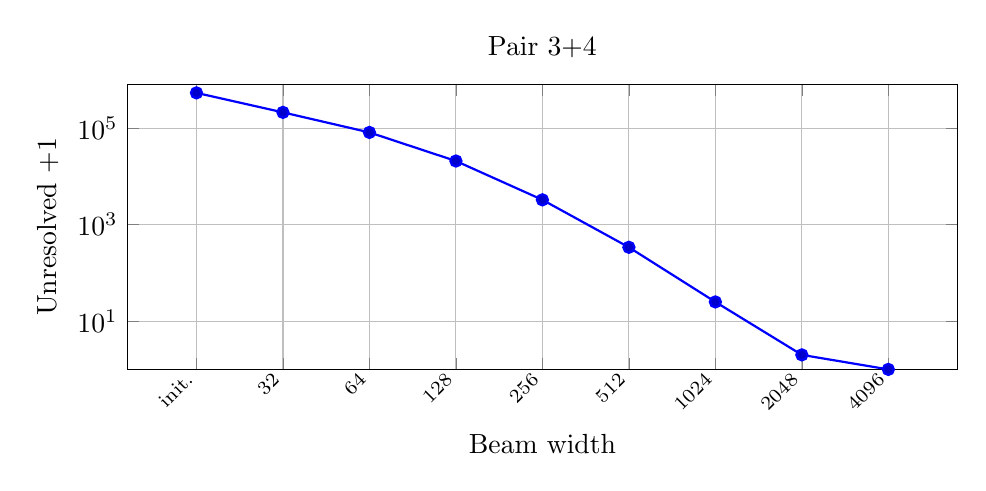
\begin{tikzpicture}
\begin{semilogyaxis}[
  width=\linewidth,height=52mm,title={Pair 3+4},
  xlabel={Beam width},ylabel={Unresolved $+1$},
  xtick={0,1,2,3,4,5,6,7,8},
  xticklabels={init.,32,64,128,256,512,1024,2048,4096},
  x tick label style={rotate=45,anchor=east,font=\scriptsize},
  ymin=1,ymax=800000,grid=major
]
\addplot+[mark=*,thick] coordinates {
  (0,536370) (1,211558) (2,81276) (3,20786) (4,3260)
  (5,339) (6,25) (7,2) (8,1)
};
\end{semilogyaxis}
\end{tikzpicture}
\end{minipage}\hfill
\begin{minipage}{0.49\linewidth}
\centering
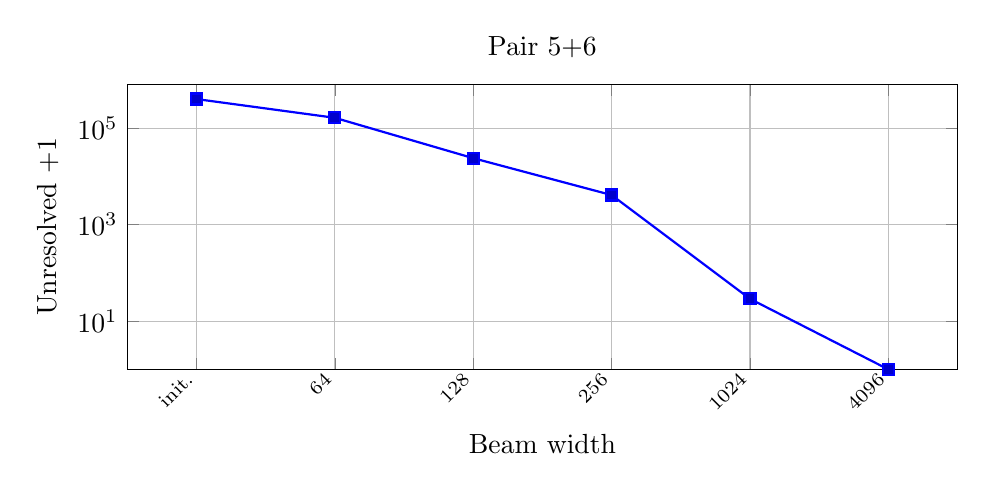
\begin{tikzpicture}
\begin{semilogyaxis}[
  width=\linewidth,height=52mm,title={Pair 5+6},
  xlabel={Beam width},ylabel={Unresolved $+1$},
  xtick={0,1,2,3,4,5},
  xticklabels={init.,64,128,256,1024,4096},
  x tick label style={rotate=45,anchor=east,font=\scriptsize},
  ymin=1,ymax=800000,grid=major
]
\addplot+[mark=square*,thick] coordinates {
  (0,399168) (1,163328) (2,23784) (3,4095) (4,29) (5,1)
};
\end{semilogyaxis}
\end{tikzpicture}
\end{minipage}
\caption{Unresolved direct-certificate obligations after each executed tier,
plotted as count plus one so that completion is represented exactly at one.
The pair-3+4 checkpoint changes within width 32; pair 5+6 changes checkpoint
between widths 64 and 128.}
\label{fig:survivor-curves}
\end{figure}

On an NVIDIA A100 80GB PCIe GPU with bfloat16 inference, active model-search
time was approximately 2~h 21~min 42~s for pair 3+4 and 3~h 53~min 44~s for
pair 5+6, or about 6~h 15~min in total.  These totals exclude phase-table
construction, exact rewriting, process gaps, and final replay.  Training logs
through the certificate-generation checkpoints record approximately 4.6
GPU-hours in total.  The point is not that every certificate had equal cost:
survivors required wider tiers in this run, and those widths were applied to
progressively smaller populations.

\begin{table}[t]
\centering
\caption{Lengths of direct neural-guided certificates.  Exact-rewrite words
are excluded.}
\label{tab:direct-word-lengths}
\small
\begin{tabular}{@{}lrrrrr@{}}
\toprule
Pair & Minimum & Median & Mean & Maximum & At maximum\\
\midrule
3+4 & 14 & 20 & 19.78 & 21 & 172,838\\
5+6 & 14 & 23 & 22.60 & 25 & 65,139\\
\bottomrule
\end{tabular}
\end{table}
These are lengths of words found by the portfolio, not shortest-distance
measurements or lower-bound witnesses.  The complete histograms appear in
\cref{app:word-lengths}.

\subsection{What the cascade data do and do not establish}

The published execution achieves complete coverage, but it is not a controlled
ablation.  Later tiers operate on distributions selected by earlier tiers, and
both pairs change checkpoint during the schedule.  Pair 3+4 also combines a
partial epoch-1024 pass with the epoch-1120 pass at width 32, while pair 5+6
changes from epoch 864 to epoch 3744 after width 64.  Consequently the rows do
not identify a pure width effect, and throughput measurements from different
tiers are not directly comparable.

We therefore make a narrower empirical claim: this particular portfolio found
bounded, independently replayable words for all 935,536 states left after exact
rewriting, within the reported hardware budget.  Establishing superiority to
IDA*, A*, a single fixed-width beam, or another learned policy would require a
separate controlled benchmark.  The certified upper bounds do not depend on
the outcome of such a comparison.

\subsection{Limitations}

The method is tailored to a one-move improvement, where only the product of
two maximal layers needs special treatment.  Larger reductions would generally
require certifying thicker boundary bands or a stronger structural argument.
The current neural targets are noisy random-walk depths, not exact distances;
the models have no admissibility guarantee.  Finally, the local bounds are
unconditional only for the two subgroup transitions reconstructed here.  The
112- and 111-move statements inherit the external assumptions made explicit in
\cref{cor:conditional-112,cor:conditional-111}.
